\documentclass[twoside]{book}

% Packages required by doxygen
\usepackage{calc}
\usepackage{doxygen}
\usepackage{graphicx}
\usepackage[utf8]{inputenc}
\usepackage{makeidx}
\usepackage{multicol}
\usepackage{multirow}
\usepackage{textcomp}
\usepackage[table]{xcolor}

% Font selection
\usepackage[T1]{fontenc}
\usepackage{mathptmx}
\usepackage[scaled=.90]{helvet}
\usepackage{courier}
\usepackage{amssymb}
\usepackage{sectsty}
\renewcommand{\familydefault}{\sfdefault}
\allsectionsfont{%
  \fontseries{bc}\selectfont%
  \color{darkgray}%
}
\renewcommand{\DoxyLabelFont}{%
  \fontseries{bc}\selectfont%
  \color{darkgray}%
}

% Page & text layout
\usepackage{geometry}
\geometry{%
  a4paper,%
  top=2.5cm,%
  bottom=2.5cm,%
  left=2.5cm,%
  right=2.5cm%
}
\tolerance=750
\hfuzz=15pt
\hbadness=750
\setlength{\emergencystretch}{15pt}
\setlength{\parindent}{0cm}
\setlength{\parskip}{0.2cm}
\makeatletter
\renewcommand{\paragraph}{%
  \@startsection{paragraph}{4}{0ex}{-1.0ex}{1.0ex}{%
    \normalfont\normalsize\bfseries\SS@parafont%
  }%
}
\renewcommand{\subparagraph}{%
  \@startsection{subparagraph}{5}{0ex}{-1.0ex}{1.0ex}{%
    \normalfont\normalsize\bfseries\SS@subparafont%
  }%
}
\makeatother

% Headers & footers
\usepackage{fancyhdr}
\pagestyle{fancyplain}
\fancyhead[LE]{\fancyplain{}{\bfseries\thepage}}
\fancyhead[CE]{\fancyplain{}{}}
\fancyhead[RE]{\fancyplain{}{\bfseries\leftmark}}
\fancyhead[LO]{\fancyplain{}{\bfseries\rightmark}}
\fancyhead[CO]{\fancyplain{}{}}
\fancyhead[RO]{\fancyplain{}{\bfseries\thepage}}
\fancyfoot[LE]{\fancyplain{}{}}
\fancyfoot[CE]{\fancyplain{}{}}
\fancyfoot[RE]{\fancyplain{}{\bfseries\scriptsize Generated on Wed Jun 19 2013 04:28:31 for Sharerd-Printing by Doxygen }}
\fancyfoot[LO]{\fancyplain{}{\bfseries\scriptsize Generated on Wed Jun 19 2013 04:28:31 for Sharerd-Printing by Doxygen }}
\fancyfoot[CO]{\fancyplain{}{}}
\fancyfoot[RO]{\fancyplain{}{}}
\renewcommand{\footrulewidth}{0.4pt}
\renewcommand{\chaptermark}[1]{%
  \markboth{#1}{}%
}
\renewcommand{\sectionmark}[1]{%
  \markright{\thesection\ #1}%
}

% Indices & bibliography
\usepackage{natbib}
\usepackage[titles]{tocloft}
\setcounter{tocdepth}{3}
\setcounter{secnumdepth}{5}
\makeindex

% Custom commands
\newcommand{\clearemptydoublepage}{%
  \newpage{\pagestyle{empty}\cleardoublepage}%
}


%===== C O N T E N T S =====

\begin{document}

% Titlepage & ToC
\pagenumbering{roman}
\begin{titlepage}
\vspace*{7cm}
\begin{center}%
{\Large Sharerd-\/\-Printing }\\
\vspace*{1cm}
{\large Generated by Doxygen 1.8.4}\\
\vspace*{0.5cm}
{\small Wed Jun 19 2013 04:28:31}\\
\end{center}
\end{titlepage}
\clearemptydoublepage
\tableofcontents
\clearemptydoublepage
\pagenumbering{arabic}

%--- Begin generated contents ---
\chapter{Namespace Index}
\section{Packages}
Here are the packages with brief descriptions (if available)\-:\begin{DoxyCompactList}
\item\contentsline{section}{{\bf client} }{\pageref{namespaceclient}}{}
\item\contentsline{section}{{\bf general} }{\pageref{namespacegeneral}}{}
\item\contentsline{section}{{\bf Printing} }{\pageref{namespace_printing}}{}
\item\contentsline{section}{{\bf Server} }{\pageref{namespace_server}}{}
\end{DoxyCompactList}

\chapter{Hierarchical Index}
\section{Class Hierarchy}
This inheritance list is sorted roughly, but not completely, alphabetically\-:\begin{DoxyCompactList}
\item \contentsline{section}{general.\-A\-Computer$<$ Tprinter, Tuser $>$}{\pageref{classgeneral_1_1_a_computer_3_01_tprinter_00_01_tuser_01_4}}{}
\begin{DoxyCompactList}
\item \contentsline{section}{general.\-Computer}{\pageref{classgeneral_1_1_computer}}{}
\end{DoxyCompactList}
\item \contentsline{section}{general.\-A\-Topology$<$ Ttransfertype $>$}{\pageref{classgeneral_1_1_a_topology_3_01_ttransfertype_01_4}}{}
\begin{DoxyCompactList}
\item \contentsline{section}{general.\-Server\-Client$<$ Ttransfertype $>$}{\pageref{classgeneral_1_1_server_client_3_01_ttransfertype_01_4}}{}
\end{DoxyCompactList}
\item \contentsline{section}{client.\-client}{\pageref{classclient_1_1client}}{}
\item \contentsline{section}{client.\-client\-G\-U\-I}{\pageref{interfaceclient_1_1client_g_u_i}}{}
\item \contentsline{section}{general.\-I\-Application}{\pageref{interfacegeneral_1_1_i_application}}{}
\begin{DoxyCompactList}
\item \contentsline{section}{Server.\-Server}{\pageref{class_server_1_1_server}}{}
\end{DoxyCompactList}
\item I\-Printer\begin{DoxyCompactList}
\item \contentsline{section}{general.\-Printer}{\pageref{classgeneral_1_1_printer}}{}
\end{DoxyCompactList}
\item \contentsline{section}{I\-Printer$<$ Ttasktype, Tstate $>$}{\pageref{interface_i_printer_3_01_ttasktype_00_01_tstate_01_4}}{}
\item \contentsline{section}{general.\-I\-Print\-Task}{\pageref{interfacegeneral_1_1_i_print_task}}{}
\begin{DoxyCompactList}
\item \contentsline{section}{general.\-Print\-Task}{\pageref{classgeneral_1_1_print_task}}{}
\end{DoxyCompactList}
\item \contentsline{section}{general.\-I\-Protocol$<$ Ttransfertype $>$}{\pageref{interfacegeneral_1_1_i_protocol_3_01_ttransfertype_01_4}}{}
\begin{DoxyCompactList}
\item \contentsline{section}{general.\-Protocol\-Soap$<$ Ttransfertype $>$}{\pageref{classgeneral_1_1_protocol_soap_3_01_ttransfertype_01_4}}{}
\end{DoxyCompactList}
\item Marshal\-By\-Ref\-Object\begin{DoxyCompactList}
\item \contentsline{section}{general.\-Printer}{\pageref{classgeneral_1_1_printer}}{}
\item \contentsline{section}{general.\-Print\-Task}{\pageref{classgeneral_1_1_print_task}}{}
\end{DoxyCompactList}
\item \contentsline{section}{Printing.\-Printing}{\pageref{class_printing_1_1_printing}}{}
\end{DoxyCompactList}

\chapter{Class Index}
\section{Class List}
Here are the classes, structs, unions and interfaces with brief descriptions\-:\begin{DoxyCompactList}
\item\contentsline{section}{{\bf general.\-A\-Computer$<$ Tprinter, Tuser $>$} }{\pageref{classgeneral_1_1_a_computer_3_01_tprinter_00_01_tuser_01_4}}{}
\item\contentsline{section}{{\bf general.\-A\-Topology$<$ Ttransfertype $>$} }{\pageref{classgeneral_1_1_a_topology_3_01_ttransfertype_01_4}}{}
\item\contentsline{section}{{\bf client.\-client} }{\pageref{classclient_1_1client}}{}
\item\contentsline{section}{{\bf client.\-client\-G\-U\-I} }{\pageref{interfaceclient_1_1client_g_u_i}}{}
\item\contentsline{section}{{\bf general.\-Computer} }{\pageref{classgeneral_1_1_computer}}{}
\item\contentsline{section}{{\bf general.\-I\-Application} }{\pageref{interfacegeneral_1_1_i_application}}{}
\item\contentsline{section}{{\bf I\-Printer$<$ Ttasktype, Tstate $>$} }{\pageref{interface_i_printer_3_01_ttasktype_00_01_tstate_01_4}}{}
\item\contentsline{section}{{\bf general.\-I\-Print\-Task} }{\pageref{interfacegeneral_1_1_i_print_task}}{}
\item\contentsline{section}{{\bf general.\-I\-Protocol$<$ Ttransfertype $>$} }{\pageref{interfacegeneral_1_1_i_protocol_3_01_ttransfertype_01_4}}{}
\item\contentsline{section}{{\bf general.\-Printer} }{\pageref{classgeneral_1_1_printer}}{}
\item\contentsline{section}{{\bf Printing.\-Printing} }{\pageref{class_printing_1_1_printing}}{}
\item\contentsline{section}{{\bf general.\-Print\-Task} }{\pageref{classgeneral_1_1_print_task}}{}
\item\contentsline{section}{{\bf general.\-Protocol\-Soap$<$ Ttransfertype $>$} }{\pageref{classgeneral_1_1_protocol_soap_3_01_ttransfertype_01_4}}{}
\item\contentsline{section}{{\bf Server.\-Server} }{\pageref{class_server_1_1_server}}{}
\item\contentsline{section}{{\bf general.\-Server\-Client$<$ Ttransfertype $>$} }{\pageref{classgeneral_1_1_server_client_3_01_ttransfertype_01_4}}{}
\end{DoxyCompactList}

\chapter{File Index}
\section{File List}
Here is a list of all files with brief descriptions\-:\begin{DoxyCompactList}
\item\contentsline{section}{{\bf main.\-cs} }{\pageref{main_8cs}}{}
\item\contentsline{section}{client/{\bf client.\-cs} }{\pageref{client_8cs}}{}
\item\contentsline{section}{client/{\bf client\-G\-U\-I.\-cs} }{\pageref{client_g_u_i_8cs}}{}
\item\contentsline{section}{general/{\bf A\-Computer.\-cs} }{\pageref{_a_computer_8cs}}{}
\item\contentsline{section}{general/{\bf Computer.\-cs} }{\pageref{_computer_8cs}}{}
\item\contentsline{section}{general/{\bf I\-Application.\-cs} }{\pageref{_i_application_8cs}}{}
\item\contentsline{section}{general/{\bf I\-Printer.\-cs} }{\pageref{_i_printer_8cs}}{}
\item\contentsline{section}{general/{\bf I\-Print\-Task.\-cs} }{\pageref{_i_print_task_8cs}}{}
\item\contentsline{section}{general/{\bf Printer.\-cs} }{\pageref{_printer_8cs}}{}
\item\contentsline{section}{general/{\bf Print\-Task.\-cs} }{\pageref{_print_task_8cs}}{}
\item\contentsline{section}{general/communication/protocol/{\bf I\-Protocol.\-cs} }{\pageref{_i_protocol_8cs}}{}
\item\contentsline{section}{general/communication/protocol/{\bf Protocol\-Soap.\-cs} }{\pageref{_protocol_soap_8cs}}{}
\item\contentsline{section}{general/communication/topology/{\bf Atopology.\-cs} }{\pageref{_atopology_8cs}}{}
\item\contentsline{section}{general/communication/topology/{\bf Server\-Client.\-cs} }{\pageref{_server_client_8cs}}{}
\item\contentsline{section}{general/\-Properties/{\bf Assembly\-Info.\-cs} }{\pageref{_assembly_info_8cs}}{}
\item\contentsline{section}{server/{\bf server.\-cs} }{\pageref{server_8cs}}{}
\end{DoxyCompactList}

\chapter{Namespace Documentation}
\section{Package client}
\label{namespaceclient}\index{client@{client}}
\subsection*{Classes}
\begin{DoxyCompactItemize}
\item 
class {\bf client}
\item 
interface {\bf client\-G\-U\-I}
\end{DoxyCompactItemize}

\section{Package general}
\label{namespacegeneral}\index{general@{general}}
\subsection*{Classes}
\begin{DoxyCompactItemize}
\item 
class {\bf A\-Computer$<$ Tprinter, Tuser $>$}
\item 
interface {\bf I\-Protocol$<$ Ttransfertype $>$}
\item 
class {\bf Protocol\-Soap$<$ Ttransfertype $>$}
\item 
class {\bf A\-Topology$<$ Ttransfertype $>$}
\item 
class {\bf Server\-Client$<$ Ttransfertype $>$}
\item 
class {\bf Computer}
\item 
interface {\bf I\-Application}
\item 
interface {\bf I\-Print\-Task}
\item 
class {\bf Printer}
\item 
class {\bf Print\-Task}
\end{DoxyCompactItemize}

\section{Package Printing}
\label{namespace_printing}\index{Printing@{Printing}}
\subsection*{Classes}
\begin{DoxyCompactItemize}
\item 
class {\bf Printing}
\end{DoxyCompactItemize}

\section{Package Server}
\label{namespace_server}\index{Server@{Server}}
\subsection*{Classes}
\begin{DoxyCompactItemize}
\item 
class {\bf Server}
\end{DoxyCompactItemize}

\chapter{Class Documentation}
\section{general.\-A\-Computer$<$ Tprinter, Tuser $>$ Class Template Reference}
\label{classgeneral_1_1_a_computer_3_01_tprinter_00_01_tuser_01_4}\index{general.\-A\-Computer$<$ Tprinter, Tuser $>$@{general.\-A\-Computer$<$ Tprinter, Tuser $>$}}
Inheritance diagram for general.\-A\-Computer$<$ Tprinter, Tuser $>$\-:\begin{figure}[H]
\begin{center}
\leavevmode
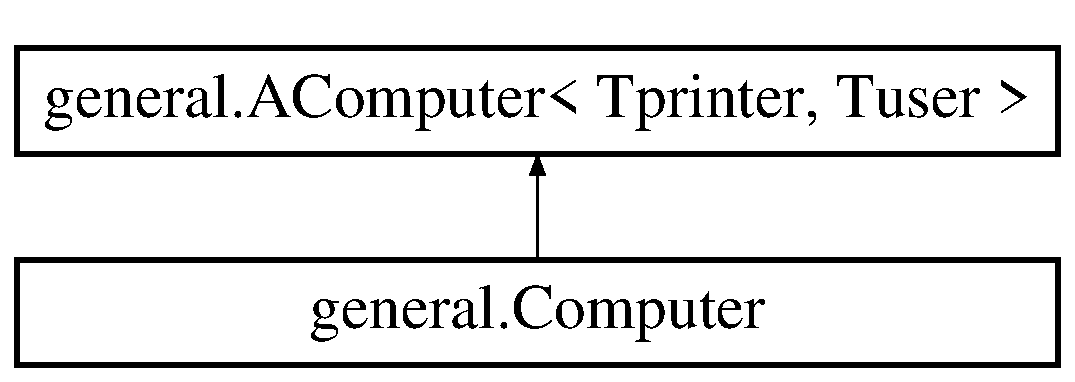
\includegraphics[height=2.000000cm]{classgeneral_1_1_a_computer_3_01_tprinter_00_01_tuser_01_4}
\end{center}
\end{figure}
\subsection*{Public Attributes}
\begin{DoxyCompactItemize}
\item 
Tprinter[$\,$] {\bf printer} = new Tprinter[2]
\item 
Tuser[$\,$] {\bf user} = new Tuser[2]
\item 
string {\bf name}
\end{DoxyCompactItemize}


\subsection{Member Data Documentation}
\index{general\-::\-A\-Computer$<$ Tprinter, Tuser $>$@{general\-::\-A\-Computer$<$ Tprinter, Tuser $>$}!name@{name}}
\index{name@{name}!general::AComputer< Tprinter, Tuser >@{general\-::\-A\-Computer$<$ Tprinter, Tuser $>$}}
\subsubsection[{name}]{\setlength{\rightskip}{0pt plus 5cm}string general.\-A\-Computer$<$ Tprinter, Tuser $>$.name}\label{classgeneral_1_1_a_computer_3_01_tprinter_00_01_tuser_01_4_a2757225751249691a992ac3131490c77}
\index{general\-::\-A\-Computer$<$ Tprinter, Tuser $>$@{general\-::\-A\-Computer$<$ Tprinter, Tuser $>$}!printer@{printer}}
\index{printer@{printer}!general::AComputer< Tprinter, Tuser >@{general\-::\-A\-Computer$<$ Tprinter, Tuser $>$}}
\subsubsection[{printer}]{\setlength{\rightskip}{0pt plus 5cm}Tprinter [$\,$] general.\-A\-Computer$<$ Tprinter, Tuser $>$.printer = new Tprinter[2]}\label{classgeneral_1_1_a_computer_3_01_tprinter_00_01_tuser_01_4_a2958528912a8e54a2996e34c7dff0f17}
\index{general\-::\-A\-Computer$<$ Tprinter, Tuser $>$@{general\-::\-A\-Computer$<$ Tprinter, Tuser $>$}!user@{user}}
\index{user@{user}!general::AComputer< Tprinter, Tuser >@{general\-::\-A\-Computer$<$ Tprinter, Tuser $>$}}
\subsubsection[{user}]{\setlength{\rightskip}{0pt plus 5cm}Tuser [$\,$] general.\-A\-Computer$<$ Tprinter, Tuser $>$.user = new Tuser[2]}\label{classgeneral_1_1_a_computer_3_01_tprinter_00_01_tuser_01_4_a01d747a58d08f2074b8960c5293875fc}


The documentation for this class was generated from the following file\-:\begin{DoxyCompactItemize}
\item 
general/{\bf A\-Computer.\-cs}\end{DoxyCompactItemize}

\section{general.\-A\-Topology$<$ Ttransfertype $>$ Class Template Reference}
\label{classgeneral_1_1_a_topology_3_01_ttransfertype_01_4}\index{general.\-A\-Topology$<$ Ttransfertype $>$@{general.\-A\-Topology$<$ Ttransfertype $>$}}
Inheritance diagram for general.\-A\-Topology$<$ Ttransfertype $>$\-:\begin{figure}[H]
\begin{center}
\leavevmode
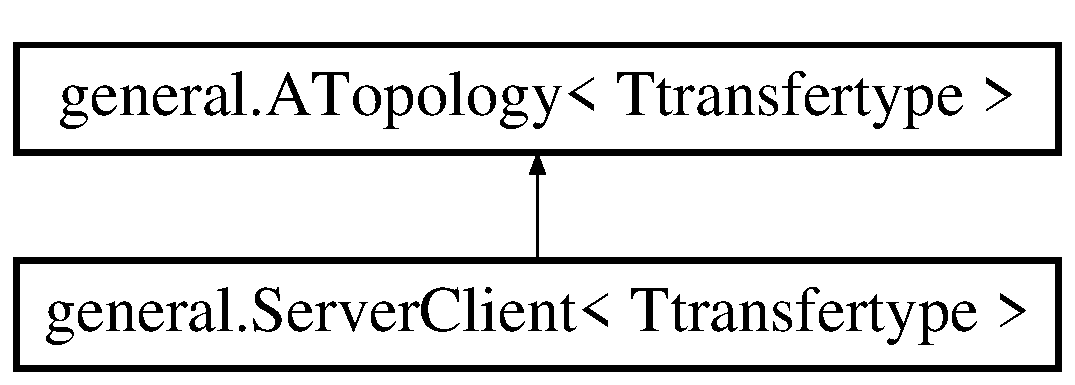
\includegraphics[height=2.000000cm]{classgeneral_1_1_a_topology_3_01_ttransfertype_01_4}
\end{center}
\end{figure}
\subsection*{Public Member Functions}
\begin{DoxyCompactItemize}
\item 
{\bf A\-Topology} (I\-Protocol$<$ Ttransfertype $>$ {\bf protocol})
\item 
abstract bool {\bf connect} (Ttransfertype obj)
\item 
abstract void {\bf disconnect} ()
\end{DoxyCompactItemize}
\subsection*{Public Attributes}
\begin{DoxyCompactItemize}
\item 
string {\bf name} = \char`\"{}Default Abstract Topology!\char`\"{}
\end{DoxyCompactItemize}
\subsection*{Protected Attributes}
\begin{DoxyCompactItemize}
\item 
I\-Protocol$<$ Ttransfertype $>$ {\bf protocol}
\end{DoxyCompactItemize}


\subsection{Constructor \& Destructor Documentation}
\index{general\-::\-A\-Topology$<$ Ttransfertype $>$@{general\-::\-A\-Topology$<$ Ttransfertype $>$}!A\-Topology@{A\-Topology}}
\index{A\-Topology@{A\-Topology}!general::ATopology< Ttransfertype >@{general\-::\-A\-Topology$<$ Ttransfertype $>$}}
\subsubsection[{A\-Topology}]{\setlength{\rightskip}{0pt plus 5cm}general.\-A\-Topology$<$ Ttransfertype $>$.A\-Topology (
\begin{DoxyParamCaption}
\item[{I\-Protocol$<$ Ttransfertype $>$}]{protocol}
\end{DoxyParamCaption}
)}\label{classgeneral_1_1_a_topology_3_01_ttransfertype_01_4_abe187cf5b67383dcd303edc9238c130f}


\subsection{Member Function Documentation}
\index{general\-::\-A\-Topology$<$ Ttransfertype $>$@{general\-::\-A\-Topology$<$ Ttransfertype $>$}!connect@{connect}}
\index{connect@{connect}!general::ATopology< Ttransfertype >@{general\-::\-A\-Topology$<$ Ttransfertype $>$}}
\subsubsection[{connect}]{\setlength{\rightskip}{0pt plus 5cm}abstract bool general.\-A\-Topology$<$ Ttransfertype $>$.connect (
\begin{DoxyParamCaption}
\item[{Ttransfertype}]{obj}
\end{DoxyParamCaption}
)\hspace{0.3cm}{\ttfamily [pure virtual]}}\label{classgeneral_1_1_a_topology_3_01_ttransfertype_01_4_ad98d6292318094e2f8e6008324adb6b6}


Implemented in {\bf general.\-Server\-Client$<$ Ttransfertype $>$} \doxyref{}{p.}{classgeneral_1_1_server_client_3_01_ttransfertype_01_4_ac79cb3704b830ad1436bb18b48ed5755}.

\index{general\-::\-A\-Topology$<$ Ttransfertype $>$@{general\-::\-A\-Topology$<$ Ttransfertype $>$}!disconnect@{disconnect}}
\index{disconnect@{disconnect}!general::ATopology< Ttransfertype >@{general\-::\-A\-Topology$<$ Ttransfertype $>$}}
\subsubsection[{disconnect}]{\setlength{\rightskip}{0pt plus 5cm}abstract void general.\-A\-Topology$<$ Ttransfertype $>$.disconnect (
\begin{DoxyParamCaption}
{}
\end{DoxyParamCaption}
)\hspace{0.3cm}{\ttfamily [pure virtual]}}\label{classgeneral_1_1_a_topology_3_01_ttransfertype_01_4_ad51a3927e211946711c52f368ce21301}


Implemented in {\bf general.\-Server\-Client$<$ Ttransfertype $>$} \doxyref{}{p.}{classgeneral_1_1_server_client_3_01_ttransfertype_01_4_a39edc8a7d4acc3c36baee5b90be87423}.



\subsection{Member Data Documentation}
\index{general\-::\-A\-Topology$<$ Ttransfertype $>$@{general\-::\-A\-Topology$<$ Ttransfertype $>$}!name@{name}}
\index{name@{name}!general::ATopology< Ttransfertype >@{general\-::\-A\-Topology$<$ Ttransfertype $>$}}
\subsubsection[{name}]{\setlength{\rightskip}{0pt plus 5cm}string general.\-A\-Topology$<$ Ttransfertype $>$.name = \char`\"{}Default Abstract Topology!\char`\"{}}\label{classgeneral_1_1_a_topology_3_01_ttransfertype_01_4_a914adb6d1d3994d9d71aa1df388c4d1d}
\index{general\-::\-A\-Topology$<$ Ttransfertype $>$@{general\-::\-A\-Topology$<$ Ttransfertype $>$}!protocol@{protocol}}
\index{protocol@{protocol}!general::ATopology< Ttransfertype >@{general\-::\-A\-Topology$<$ Ttransfertype $>$}}
\subsubsection[{protocol}]{\setlength{\rightskip}{0pt plus 5cm}I\-Protocol$<$Ttransfertype$>$ general.\-A\-Topology$<$ Ttransfertype $>$.protocol\hspace{0.3cm}{\ttfamily [protected]}}\label{classgeneral_1_1_a_topology_3_01_ttransfertype_01_4_aa9fe2e70cf933ceafaa6fa0c16710836}


The documentation for this class was generated from the following file\-:\begin{DoxyCompactItemize}
\item 
general/communication/topology/{\bf Atopology.\-cs}\end{DoxyCompactItemize}

\section{client.\-client Class Reference}
\label{classclient_1_1client}\index{client.\-client@{client.\-client}}


The documentation for this class was generated from the following file\-:\begin{DoxyCompactItemize}
\item 
client/{\bf client.\-cs}\end{DoxyCompactItemize}

\section{client.\-client\-G\-U\-I Interface Reference}
\label{interfaceclient_1_1client_g_u_i}\index{client.\-client\-G\-U\-I@{client.\-client\-G\-U\-I}}


The documentation for this interface was generated from the following file\-:\begin{DoxyCompactItemize}
\item 
client/{\bf client\-G\-U\-I.\-cs}\end{DoxyCompactItemize}

\section{general.\-Computer Class Reference}
\label{classgeneral_1_1_computer}\index{general.\-Computer@{general.\-Computer}}
Inheritance diagram for general.\-Computer\-:\begin{figure}[H]
\begin{center}
\leavevmode
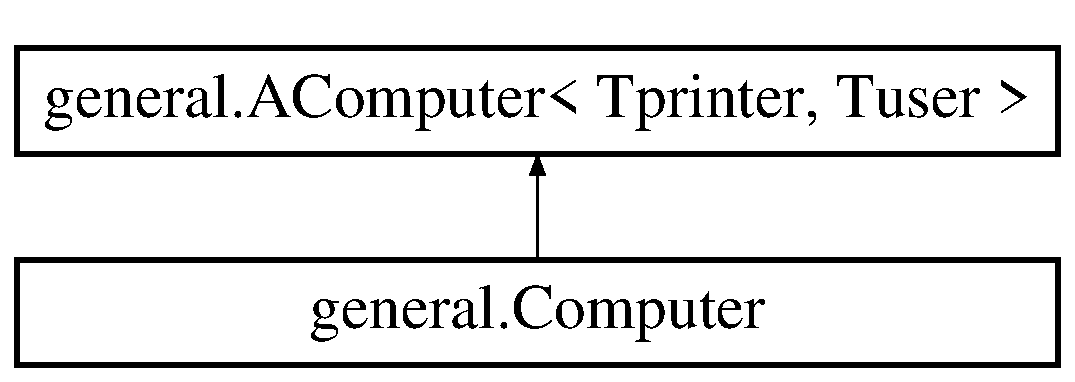
\includegraphics[height=2.000000cm]{classgeneral_1_1_computer}
\end{center}
\end{figure}
\subsection*{Additional Inherited Members}


The documentation for this class was generated from the following file\-:\begin{DoxyCompactItemize}
\item 
general/{\bf Computer.\-cs}\end{DoxyCompactItemize}

\section{general.\-I\-Application Interface Reference}
\label{interfacegeneral_1_1_i_application}\index{general.\-I\-Application@{general.\-I\-Application}}
Inheritance diagram for general.\-I\-Application\-:\begin{figure}[H]
\begin{center}
\leavevmode
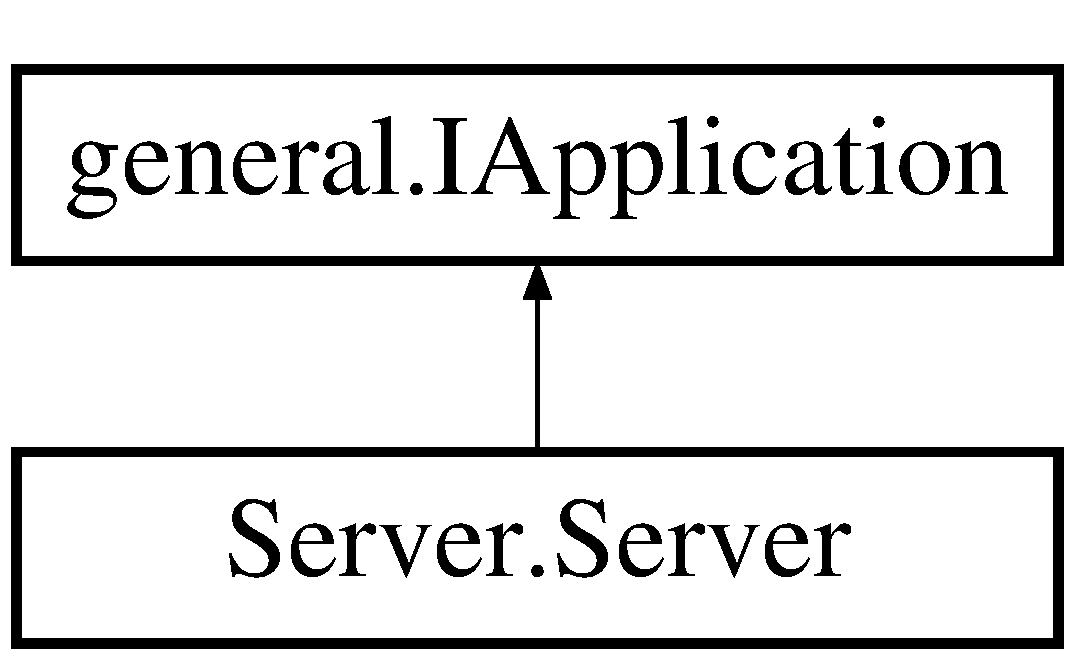
\includegraphics[height=2.000000cm]{interfacegeneral_1_1_i_application}
\end{center}
\end{figure}
\subsection*{Public Member Functions}
\begin{DoxyCompactItemize}
\item 
bool {\bf init} ()
\item 
bool {\bf start} ()
\item 
bool {\bf stop} ()
\end{DoxyCompactItemize}


\subsection{Member Function Documentation}
\index{general\-::\-I\-Application@{general\-::\-I\-Application}!init@{init}}
\index{init@{init}!general::IApplication@{general\-::\-I\-Application}}
\subsubsection[{init}]{\setlength{\rightskip}{0pt plus 5cm}bool general.\-I\-Application.\-init (
\begin{DoxyParamCaption}
{}
\end{DoxyParamCaption}
)}\label{interfacegeneral_1_1_i_application_a0b53a00ac509c31efcc46fe5d20c156f}
Initialize Application object +\-Do any pre setting up before application starts +\-Should include things not critical to the creation of the object. 

Implemented in {\bf Server.\-Server} \doxyref{}{p.}{class_server_1_1_server_afb8a142170af0d8758ca23875bc93d69}.

\index{general\-::\-I\-Application@{general\-::\-I\-Application}!start@{start}}
\index{start@{start}!general::IApplication@{general\-::\-I\-Application}}
\subsubsection[{start}]{\setlength{\rightskip}{0pt plus 5cm}bool general.\-I\-Application.\-start (
\begin{DoxyParamCaption}
{}
\end{DoxyParamCaption}
)}\label{interfacegeneral_1_1_i_application_a44ef333a6aefd814ef4db3f04a45b5e1}
Start application 

Implemented in {\bf Server.\-Server} \doxyref{}{p.}{class_server_1_1_server_a161ab2103af04dcdd6d00645a3072d30}.

\index{general\-::\-I\-Application@{general\-::\-I\-Application}!stop@{stop}}
\index{stop@{stop}!general::IApplication@{general\-::\-I\-Application}}
\subsubsection[{stop}]{\setlength{\rightskip}{0pt plus 5cm}bool general.\-I\-Application.\-stop (
\begin{DoxyParamCaption}
{}
\end{DoxyParamCaption}
)}\label{interfacegeneral_1_1_i_application_a497ef4a13f7f98a1a7656c529933fa53}
Stop application +\-Should return true on successful stop. +\-Should only stop if application is not busy, in this case return false. 

Implemented in {\bf Server.\-Server} \doxyref{}{p.}{class_server_1_1_server_a84955f96214411a79da90cd2acfd7e2d}.



The documentation for this interface was generated from the following file\-:\begin{DoxyCompactItemize}
\item 
general/{\bf I\-Application.\-cs}\end{DoxyCompactItemize}

\section{I\-Printer$<$ Ttasktype, Tstate $>$ Interface Template Reference}
\label{interface_i_printer_3_01_ttasktype_00_01_tstate_01_4}\index{I\-Printer$<$ Ttasktype, Tstate $>$@{I\-Printer$<$ Ttasktype, Tstate $>$}}
\subsection*{Public Member Functions}
\begin{DoxyCompactItemize}
\item 
string {\bf get\-Type} ()
\item 
Tstate {\bf get\-State} ()
\end{DoxyCompactItemize}


\subsection{Member Function Documentation}
\index{I\-Printer$<$ Ttasktype, Tstate $>$@{I\-Printer$<$ Ttasktype, Tstate $>$}!get\-State@{get\-State}}
\index{get\-State@{get\-State}!IPrinter< Ttasktype, Tstate >@{I\-Printer$<$ Ttasktype, Tstate $>$}}
\subsubsection[{get\-State}]{\setlength{\rightskip}{0pt plus 5cm}Tstate I\-Printer$<$ Ttasktype, Tstate $>$.get\-State (
\begin{DoxyParamCaption}
{}
\end{DoxyParamCaption}
)}\label{interface_i_printer_3_01_ttasktype_00_01_tstate_01_4_af00bcb55311b60e29f77fdbdf92275b2}
\index{I\-Printer$<$ Ttasktype, Tstate $>$@{I\-Printer$<$ Ttasktype, Tstate $>$}!get\-Type@{get\-Type}}
\index{get\-Type@{get\-Type}!IPrinter< Ttasktype, Tstate >@{I\-Printer$<$ Ttasktype, Tstate $>$}}
\subsubsection[{get\-Type}]{\setlength{\rightskip}{0pt plus 5cm}string I\-Printer$<$ Ttasktype, Tstate $>$.get\-Type (
\begin{DoxyParamCaption}
{}
\end{DoxyParamCaption}
)}\label{interface_i_printer_3_01_ttasktype_00_01_tstate_01_4_a5bd7a982069ca4f4da8633b18f5bacd8}


The documentation for this interface was generated from the following file\-:\begin{DoxyCompactItemize}
\item 
general/{\bf I\-Printer.\-cs}\end{DoxyCompactItemize}

\section{general.\-I\-Print\-Task Interface Reference}
\label{interfacegeneral_1_1_i_print_task}\index{general.\-I\-Print\-Task@{general.\-I\-Print\-Task}}
Inheritance diagram for general.\-I\-Print\-Task\-:\begin{figure}[H]
\begin{center}
\leavevmode
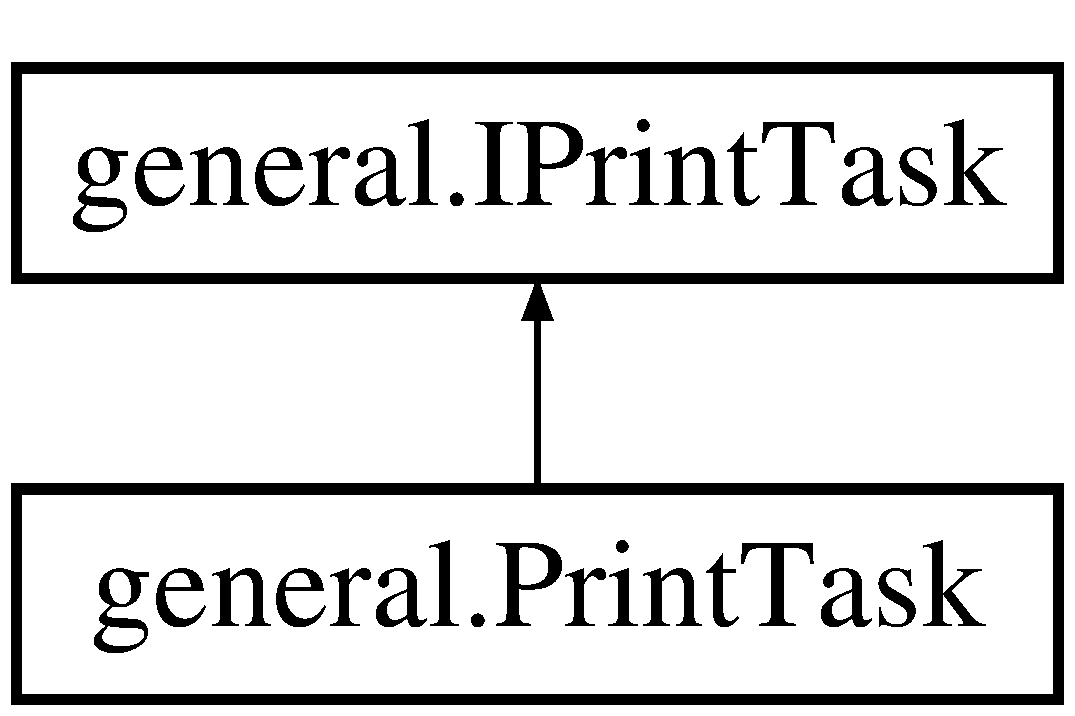
\includegraphics[height=2.000000cm]{interfacegeneral_1_1_i_print_task}
\end{center}
\end{figure}
\subsection*{Public Member Functions}
\begin{DoxyCompactItemize}
\item 
void {\bf Set\-Print\-Task} (string user\-Name, string print\-Name, int print\-Copies)
\item 
String {\bf Get\-User\-Name} ()
\item 
void {\bf Set\-User\-Name} (string name)
\item 
String {\bf Get\-Print\-Name} ()
\item 
void {\bf Set\-Print\-Name} (string name)
\item 
int {\bf Get\-Copies} ()
\item 
void {\bf Set\-Copies} (int copies)
\end{DoxyCompactItemize}


\subsection{Member Function Documentation}
\index{general\-::\-I\-Print\-Task@{general\-::\-I\-Print\-Task}!Get\-Copies@{Get\-Copies}}
\index{Get\-Copies@{Get\-Copies}!general::IPrintTask@{general\-::\-I\-Print\-Task}}
\subsubsection[{Get\-Copies}]{\setlength{\rightskip}{0pt plus 5cm}int general.\-I\-Print\-Task.\-Get\-Copies (
\begin{DoxyParamCaption}
{}
\end{DoxyParamCaption}
)}\label{interfacegeneral_1_1_i_print_task_adbd8cb47159d8067e2ad50c7dbd4605c}


Implemented in {\bf general.\-Print\-Task} \doxyref{}{p.}{classgeneral_1_1_print_task_a4a815fd603038c9456433d9dbc6cd6d4}.

\index{general\-::\-I\-Print\-Task@{general\-::\-I\-Print\-Task}!Get\-Print\-Name@{Get\-Print\-Name}}
\index{Get\-Print\-Name@{Get\-Print\-Name}!general::IPrintTask@{general\-::\-I\-Print\-Task}}
\subsubsection[{Get\-Print\-Name}]{\setlength{\rightskip}{0pt plus 5cm}String general.\-I\-Print\-Task.\-Get\-Print\-Name (
\begin{DoxyParamCaption}
{}
\end{DoxyParamCaption}
)}\label{interfacegeneral_1_1_i_print_task_ad47524f76cf88e6ab00709fc29433919}


Implemented in {\bf general.\-Print\-Task} \doxyref{}{p.}{classgeneral_1_1_print_task_a700a35044e3dcad226e210bd68494856}.

\index{general\-::\-I\-Print\-Task@{general\-::\-I\-Print\-Task}!Get\-User\-Name@{Get\-User\-Name}}
\index{Get\-User\-Name@{Get\-User\-Name}!general::IPrintTask@{general\-::\-I\-Print\-Task}}
\subsubsection[{Get\-User\-Name}]{\setlength{\rightskip}{0pt plus 5cm}String general.\-I\-Print\-Task.\-Get\-User\-Name (
\begin{DoxyParamCaption}
{}
\end{DoxyParamCaption}
)}\label{interfacegeneral_1_1_i_print_task_aa374f737890ac7451b43466971d1e2e2}


Implemented in {\bf general.\-Print\-Task} \doxyref{}{p.}{classgeneral_1_1_print_task_ac339b19a713df50bd1a024bf890dc0f1}.

\index{general\-::\-I\-Print\-Task@{general\-::\-I\-Print\-Task}!Set\-Copies@{Set\-Copies}}
\index{Set\-Copies@{Set\-Copies}!general::IPrintTask@{general\-::\-I\-Print\-Task}}
\subsubsection[{Set\-Copies}]{\setlength{\rightskip}{0pt plus 5cm}void general.\-I\-Print\-Task.\-Set\-Copies (
\begin{DoxyParamCaption}
\item[{int}]{copies}
\end{DoxyParamCaption}
)}\label{interfacegeneral_1_1_i_print_task_a12cb98d10b2563d1af62598ed605cda3}


Implemented in {\bf general.\-Print\-Task} \doxyref{}{p.}{classgeneral_1_1_print_task_ae070eae77b0f39a8284ab2bd67de2b18}.

\index{general\-::\-I\-Print\-Task@{general\-::\-I\-Print\-Task}!Set\-Print\-Name@{Set\-Print\-Name}}
\index{Set\-Print\-Name@{Set\-Print\-Name}!general::IPrintTask@{general\-::\-I\-Print\-Task}}
\subsubsection[{Set\-Print\-Name}]{\setlength{\rightskip}{0pt plus 5cm}void general.\-I\-Print\-Task.\-Set\-Print\-Name (
\begin{DoxyParamCaption}
\item[{string}]{name}
\end{DoxyParamCaption}
)}\label{interfacegeneral_1_1_i_print_task_af8c7c18af1e8c0b9572b4899efaae197}


Implemented in {\bf general.\-Print\-Task} \doxyref{}{p.}{classgeneral_1_1_print_task_aa8cd63d37f3f712189d6f682b7c8eb7d}.

\index{general\-::\-I\-Print\-Task@{general\-::\-I\-Print\-Task}!Set\-Print\-Task@{Set\-Print\-Task}}
\index{Set\-Print\-Task@{Set\-Print\-Task}!general::IPrintTask@{general\-::\-I\-Print\-Task}}
\subsubsection[{Set\-Print\-Task}]{\setlength{\rightskip}{0pt plus 5cm}void general.\-I\-Print\-Task.\-Set\-Print\-Task (
\begin{DoxyParamCaption}
\item[{string}]{user\-Name, }
\item[{string}]{print\-Name, }
\item[{int}]{print\-Copies}
\end{DoxyParamCaption}
)}\label{interfacegeneral_1_1_i_print_task_a869ccbcaa6eb242b8a1282a3048279ea}


Implemented in {\bf general.\-Print\-Task} \doxyref{}{p.}{classgeneral_1_1_print_task_aa82565ecbe842cdfe40af0373fa1a434}.

\index{general\-::\-I\-Print\-Task@{general\-::\-I\-Print\-Task}!Set\-User\-Name@{Set\-User\-Name}}
\index{Set\-User\-Name@{Set\-User\-Name}!general::IPrintTask@{general\-::\-I\-Print\-Task}}
\subsubsection[{Set\-User\-Name}]{\setlength{\rightskip}{0pt plus 5cm}void general.\-I\-Print\-Task.\-Set\-User\-Name (
\begin{DoxyParamCaption}
\item[{string}]{name}
\end{DoxyParamCaption}
)}\label{interfacegeneral_1_1_i_print_task_a70295277bddc966f5e81d541f008810f}


Implemented in {\bf general.\-Print\-Task} \doxyref{}{p.}{classgeneral_1_1_print_task_a057f7facea1dd68d7dcacc1f6f001017}.



The documentation for this interface was generated from the following file\-:\begin{DoxyCompactItemize}
\item 
general/{\bf I\-Print\-Task.\-cs}\end{DoxyCompactItemize}

\section{general.\-I\-Protocol$<$ Ttransfertype $>$ Interface Template Reference}
\label{interfacegeneral_1_1_i_protocol_3_01_ttransfertype_01_4}\index{general.\-I\-Protocol$<$ Ttransfertype $>$@{general.\-I\-Protocol$<$ Ttransfertype $>$}}
Inheritance diagram for general.\-I\-Protocol$<$ Ttransfertype $>$\-:\begin{figure}[H]
\begin{center}
\leavevmode
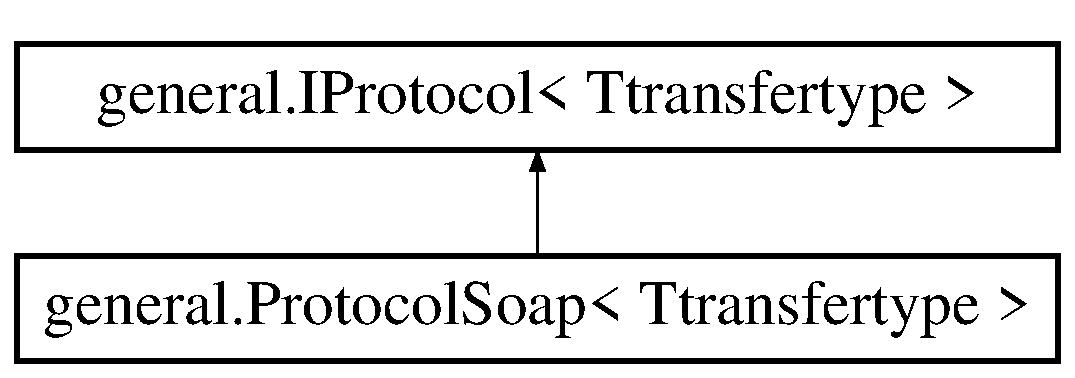
\includegraphics[height=2.000000cm]{interfacegeneral_1_1_i_protocol_3_01_ttransfertype_01_4}
\end{center}
\end{figure}
\subsection*{Public Member Functions}
\begin{DoxyCompactItemize}
\item 
bool {\bf connect} (Ttransfertype obj, string url)
\item 
void {\bf disconnect} ()
\item 
bool {\bf send} (Ttransfertype obj)
\end{DoxyCompactItemize}


\subsection{Member Function Documentation}
\index{general\-::\-I\-Protocol$<$ Ttransfertype $>$@{general\-::\-I\-Protocol$<$ Ttransfertype $>$}!connect@{connect}}
\index{connect@{connect}!general::IProtocol< Ttransfertype >@{general\-::\-I\-Protocol$<$ Ttransfertype $>$}}
\subsubsection[{connect}]{\setlength{\rightskip}{0pt plus 5cm}bool general.\-I\-Protocol$<$ Ttransfertype $>$.connect (
\begin{DoxyParamCaption}
\item[{Ttransfertype}]{obj, }
\item[{string}]{url}
\end{DoxyParamCaption}
)}\label{interfacegeneral_1_1_i_protocol_3_01_ttransfertype_01_4_add439e3269ed0417c7d31f543293cf6d}


Implemented in {\bf general.\-Protocol\-Soap$<$ Ttransfertype $>$} \doxyref{}{p.}{classgeneral_1_1_protocol_soap_3_01_ttransfertype_01_4_a14618cf7ac8a000cca11a1b4ba6771b2}.

\index{general\-::\-I\-Protocol$<$ Ttransfertype $>$@{general\-::\-I\-Protocol$<$ Ttransfertype $>$}!disconnect@{disconnect}}
\index{disconnect@{disconnect}!general::IProtocol< Ttransfertype >@{general\-::\-I\-Protocol$<$ Ttransfertype $>$}}
\subsubsection[{disconnect}]{\setlength{\rightskip}{0pt plus 5cm}void general.\-I\-Protocol$<$ Ttransfertype $>$.disconnect (
\begin{DoxyParamCaption}
{}
\end{DoxyParamCaption}
)}\label{interfacegeneral_1_1_i_protocol_3_01_ttransfertype_01_4_a21e9034c26aa630c374af028eb0e1c19}


Implemented in {\bf general.\-Protocol\-Soap$<$ Ttransfertype $>$} \doxyref{}{p.}{classgeneral_1_1_protocol_soap_3_01_ttransfertype_01_4_a08c49370d9f9c01ddee71446fe2ac072}.

\index{general\-::\-I\-Protocol$<$ Ttransfertype $>$@{general\-::\-I\-Protocol$<$ Ttransfertype $>$}!send@{send}}
\index{send@{send}!general::IProtocol< Ttransfertype >@{general\-::\-I\-Protocol$<$ Ttransfertype $>$}}
\subsubsection[{send}]{\setlength{\rightskip}{0pt plus 5cm}bool general.\-I\-Protocol$<$ Ttransfertype $>$.send (
\begin{DoxyParamCaption}
\item[{Ttransfertype}]{obj}
\end{DoxyParamCaption}
)}\label{interfacegeneral_1_1_i_protocol_3_01_ttransfertype_01_4_afb16cb0284cb948a2af24f2bd5c1b192}


Implemented in {\bf general.\-Protocol\-Soap$<$ Ttransfertype $>$} \doxyref{}{p.}{classgeneral_1_1_protocol_soap_3_01_ttransfertype_01_4_aff8117875ae68eb4b55d224e751b8ec1}.



The documentation for this interface was generated from the following file\-:\begin{DoxyCompactItemize}
\item 
general/communication/protocol/{\bf I\-Protocol.\-cs}\end{DoxyCompactItemize}

\section{general.\-Printer Class Reference}
\label{classgeneral_1_1_printer}\index{general.\-Printer@{general.\-Printer}}
Inheritance diagram for general.\-Printer\-:\begin{figure}[H]
\begin{center}
\leavevmode
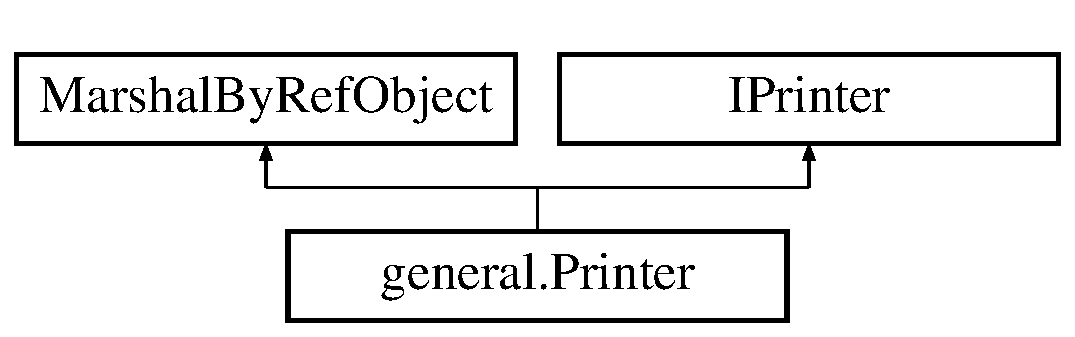
\includegraphics[height=2.000000cm]{classgeneral_1_1_printer}
\end{center}
\end{figure}
\subsection*{Public Member Functions}
\begin{DoxyCompactItemize}
\item 
{\bf Printer} ()
\item 
{\bf Printer} (string {\bf printer\-Name})
\item 
string {\bf Get\-Printer\-Name} ()
\item 
void {\bf Set\-Printer\-Name} (string name)
\item 
bool {\bf Check\-Idle} ()
\item 
void {\bf Load\-Print\-Task} (string print\-Name)
\item 
void {\bf Print} ()
\end{DoxyCompactItemize}
\subsection*{Public Attributes}
\begin{DoxyCompactItemize}
\item 
string {\bf printer\-Name}
\end{DoxyCompactItemize}


\subsection{Constructor \& Destructor Documentation}
\index{general\-::\-Printer@{general\-::\-Printer}!Printer@{Printer}}
\index{Printer@{Printer}!general::Printer@{general\-::\-Printer}}
\subsubsection[{Printer}]{\setlength{\rightskip}{0pt plus 5cm}general.\-Printer.\-Printer (
\begin{DoxyParamCaption}
{}
\end{DoxyParamCaption}
)}\label{classgeneral_1_1_printer_a8a5efd620a05ac28d8900a92ea31e1e6}
\index{general\-::\-Printer@{general\-::\-Printer}!Printer@{Printer}}
\index{Printer@{Printer}!general::Printer@{general\-::\-Printer}}
\subsubsection[{Printer}]{\setlength{\rightskip}{0pt plus 5cm}general.\-Printer.\-Printer (
\begin{DoxyParamCaption}
\item[{string}]{printer\-Name}
\end{DoxyParamCaption}
)}\label{classgeneral_1_1_printer_acbd90710c0a190c37c22cd1682df5175}


\subsection{Member Function Documentation}
\index{general\-::\-Printer@{general\-::\-Printer}!Check\-Idle@{Check\-Idle}}
\index{Check\-Idle@{Check\-Idle}!general::Printer@{general\-::\-Printer}}
\subsubsection[{Check\-Idle}]{\setlength{\rightskip}{0pt plus 5cm}bool general.\-Printer.\-Check\-Idle (
\begin{DoxyParamCaption}
{}
\end{DoxyParamCaption}
)}\label{classgeneral_1_1_printer_a7864a34ad69b6a24a6141d8965a5461a}
\index{general\-::\-Printer@{general\-::\-Printer}!Get\-Printer\-Name@{Get\-Printer\-Name}}
\index{Get\-Printer\-Name@{Get\-Printer\-Name}!general::Printer@{general\-::\-Printer}}
\subsubsection[{Get\-Printer\-Name}]{\setlength{\rightskip}{0pt plus 5cm}string general.\-Printer.\-Get\-Printer\-Name (
\begin{DoxyParamCaption}
{}
\end{DoxyParamCaption}
)}\label{classgeneral_1_1_printer_a9afebe239ae0a38bf0e7611e540986d0}
\index{general\-::\-Printer@{general\-::\-Printer}!Load\-Print\-Task@{Load\-Print\-Task}}
\index{Load\-Print\-Task@{Load\-Print\-Task}!general::Printer@{general\-::\-Printer}}
\subsubsection[{Load\-Print\-Task}]{\setlength{\rightskip}{0pt plus 5cm}void general.\-Printer.\-Load\-Print\-Task (
\begin{DoxyParamCaption}
\item[{string}]{print\-Name}
\end{DoxyParamCaption}
)}\label{classgeneral_1_1_printer_a5eeae884bd3c18be013cd11ae47c57b6}
\index{general\-::\-Printer@{general\-::\-Printer}!Print@{Print}}
\index{Print@{Print}!general::Printer@{general\-::\-Printer}}
\subsubsection[{Print}]{\setlength{\rightskip}{0pt plus 5cm}void general.\-Printer.\-Print (
\begin{DoxyParamCaption}
{}
\end{DoxyParamCaption}
)}\label{classgeneral_1_1_printer_a4f37fda001f50f3dd78d92c8370a1856}
\index{general\-::\-Printer@{general\-::\-Printer}!Set\-Printer\-Name@{Set\-Printer\-Name}}
\index{Set\-Printer\-Name@{Set\-Printer\-Name}!general::Printer@{general\-::\-Printer}}
\subsubsection[{Set\-Printer\-Name}]{\setlength{\rightskip}{0pt plus 5cm}void general.\-Printer.\-Set\-Printer\-Name (
\begin{DoxyParamCaption}
\item[{string}]{name}
\end{DoxyParamCaption}
)}\label{classgeneral_1_1_printer_a09edb8deaba3af36f8edc7ab80a11af3}


\subsection{Member Data Documentation}
\index{general\-::\-Printer@{general\-::\-Printer}!printer\-Name@{printer\-Name}}
\index{printer\-Name@{printer\-Name}!general::Printer@{general\-::\-Printer}}
\subsubsection[{printer\-Name}]{\setlength{\rightskip}{0pt plus 5cm}string general.\-Printer.\-printer\-Name}\label{classgeneral_1_1_printer_accfe10173f1a51d483fb1d2ca5a85f8e}


The documentation for this class was generated from the following file\-:\begin{DoxyCompactItemize}
\item 
general/{\bf Printer.\-cs}\end{DoxyCompactItemize}

\section{Printing.\-Printing Class Reference}
\label{class_printing_1_1_printing}\index{Printing.\-Printing@{Printing.\-Printing}}


The documentation for this class was generated from the following file\-:\begin{DoxyCompactItemize}
\item 
{\bf main.\-cs}\end{DoxyCompactItemize}

\section{general.\-Print\-Task Class Reference}
\label{classgeneral_1_1_print_task}\index{general.\-Print\-Task@{general.\-Print\-Task}}
Inheritance diagram for general.\-Print\-Task\-:\begin{figure}[H]
\begin{center}
\leavevmode
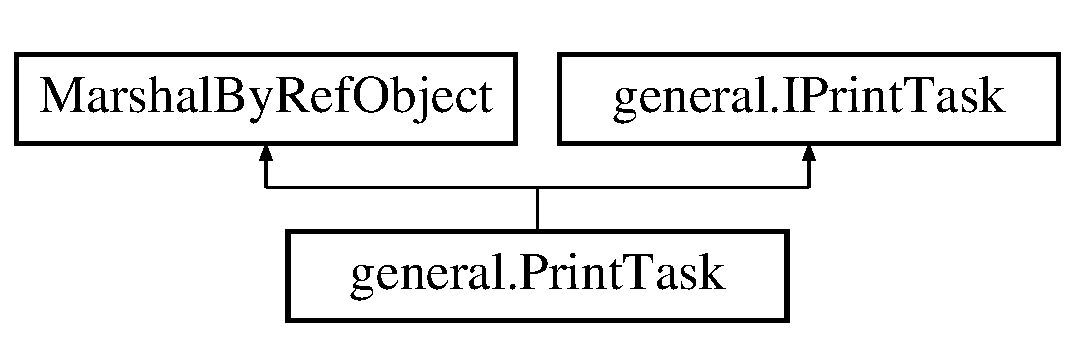
\includegraphics[height=2.000000cm]{classgeneral_1_1_print_task}
\end{center}
\end{figure}
\subsection*{Public Member Functions}
\begin{DoxyCompactItemize}
\item 
{\bf Print\-Task} ()
\item 
{\bf Print\-Task} (string user\-Name, string print\-Name, int print\-Copies)
\item 
void {\bf Set\-Print\-Task} (string user\-Name, string print\-Name, int print\-Copies)
\item 
string {\bf Get\-User\-Name} ()
\item 
void {\bf Set\-User\-Name} (string name)
\item 
string {\bf Get\-Print\-Name} ()
\item 
void {\bf Set\-Print\-Name} (string name)
\item 
int {\bf Get\-Copies} ()
\item 
void {\bf Set\-Copies} (int copies)
\end{DoxyCompactItemize}


\subsection{Constructor \& Destructor Documentation}
\index{general\-::\-Print\-Task@{general\-::\-Print\-Task}!Print\-Task@{Print\-Task}}
\index{Print\-Task@{Print\-Task}!general::PrintTask@{general\-::\-Print\-Task}}
\subsubsection[{Print\-Task}]{\setlength{\rightskip}{0pt plus 5cm}general.\-Print\-Task.\-Print\-Task (
\begin{DoxyParamCaption}
{}
\end{DoxyParamCaption}
)}\label{classgeneral_1_1_print_task_a22059cda8e02d2dca371c97310f295f3}
\index{general\-::\-Print\-Task@{general\-::\-Print\-Task}!Print\-Task@{Print\-Task}}
\index{Print\-Task@{Print\-Task}!general::PrintTask@{general\-::\-Print\-Task}}
\subsubsection[{Print\-Task}]{\setlength{\rightskip}{0pt plus 5cm}general.\-Print\-Task.\-Print\-Task (
\begin{DoxyParamCaption}
\item[{string}]{user\-Name, }
\item[{string}]{print\-Name, }
\item[{int}]{print\-Copies}
\end{DoxyParamCaption}
)}\label{classgeneral_1_1_print_task_a086539e46ffae0f944de374fe63974a3}


\subsection{Member Function Documentation}
\index{general\-::\-Print\-Task@{general\-::\-Print\-Task}!Get\-Copies@{Get\-Copies}}
\index{Get\-Copies@{Get\-Copies}!general::PrintTask@{general\-::\-Print\-Task}}
\subsubsection[{Get\-Copies}]{\setlength{\rightskip}{0pt plus 5cm}int general.\-Print\-Task.\-Get\-Copies (
\begin{DoxyParamCaption}
{}
\end{DoxyParamCaption}
)}\label{classgeneral_1_1_print_task_a4a815fd603038c9456433d9dbc6cd6d4}


Implements {\bf general.\-I\-Print\-Task} \doxyref{}{p.}{interfacegeneral_1_1_i_print_task_adbd8cb47159d8067e2ad50c7dbd4605c}.

\index{general\-::\-Print\-Task@{general\-::\-Print\-Task}!Get\-Print\-Name@{Get\-Print\-Name}}
\index{Get\-Print\-Name@{Get\-Print\-Name}!general::PrintTask@{general\-::\-Print\-Task}}
\subsubsection[{Get\-Print\-Name}]{\setlength{\rightskip}{0pt plus 5cm}string general.\-Print\-Task.\-Get\-Print\-Name (
\begin{DoxyParamCaption}
{}
\end{DoxyParamCaption}
)}\label{classgeneral_1_1_print_task_a700a35044e3dcad226e210bd68494856}


Implements {\bf general.\-I\-Print\-Task} \doxyref{}{p.}{interfacegeneral_1_1_i_print_task_ad47524f76cf88e6ab00709fc29433919}.

\index{general\-::\-Print\-Task@{general\-::\-Print\-Task}!Get\-User\-Name@{Get\-User\-Name}}
\index{Get\-User\-Name@{Get\-User\-Name}!general::PrintTask@{general\-::\-Print\-Task}}
\subsubsection[{Get\-User\-Name}]{\setlength{\rightskip}{0pt plus 5cm}string general.\-Print\-Task.\-Get\-User\-Name (
\begin{DoxyParamCaption}
{}
\end{DoxyParamCaption}
)}\label{classgeneral_1_1_print_task_ac339b19a713df50bd1a024bf890dc0f1}


Implements {\bf general.\-I\-Print\-Task} \doxyref{}{p.}{interfacegeneral_1_1_i_print_task_aa374f737890ac7451b43466971d1e2e2}.

\index{general\-::\-Print\-Task@{general\-::\-Print\-Task}!Set\-Copies@{Set\-Copies}}
\index{Set\-Copies@{Set\-Copies}!general::PrintTask@{general\-::\-Print\-Task}}
\subsubsection[{Set\-Copies}]{\setlength{\rightskip}{0pt plus 5cm}void general.\-Print\-Task.\-Set\-Copies (
\begin{DoxyParamCaption}
\item[{int}]{copies}
\end{DoxyParamCaption}
)}\label{classgeneral_1_1_print_task_ae070eae77b0f39a8284ab2bd67de2b18}


Implements {\bf general.\-I\-Print\-Task} \doxyref{}{p.}{interfacegeneral_1_1_i_print_task_a12cb98d10b2563d1af62598ed605cda3}.

\index{general\-::\-Print\-Task@{general\-::\-Print\-Task}!Set\-Print\-Name@{Set\-Print\-Name}}
\index{Set\-Print\-Name@{Set\-Print\-Name}!general::PrintTask@{general\-::\-Print\-Task}}
\subsubsection[{Set\-Print\-Name}]{\setlength{\rightskip}{0pt plus 5cm}void general.\-Print\-Task.\-Set\-Print\-Name (
\begin{DoxyParamCaption}
\item[{string}]{name}
\end{DoxyParamCaption}
)}\label{classgeneral_1_1_print_task_aa8cd63d37f3f712189d6f682b7c8eb7d}


Implements {\bf general.\-I\-Print\-Task} \doxyref{}{p.}{interfacegeneral_1_1_i_print_task_af8c7c18af1e8c0b9572b4899efaae197}.

\index{general\-::\-Print\-Task@{general\-::\-Print\-Task}!Set\-Print\-Task@{Set\-Print\-Task}}
\index{Set\-Print\-Task@{Set\-Print\-Task}!general::PrintTask@{general\-::\-Print\-Task}}
\subsubsection[{Set\-Print\-Task}]{\setlength{\rightskip}{0pt plus 5cm}void general.\-Print\-Task.\-Set\-Print\-Task (
\begin{DoxyParamCaption}
\item[{string}]{user\-Name, }
\item[{string}]{print\-Name, }
\item[{int}]{print\-Copies}
\end{DoxyParamCaption}
)}\label{classgeneral_1_1_print_task_aa82565ecbe842cdfe40af0373fa1a434}


Implements {\bf general.\-I\-Print\-Task} \doxyref{}{p.}{interfacegeneral_1_1_i_print_task_a869ccbcaa6eb242b8a1282a3048279ea}.

\index{general\-::\-Print\-Task@{general\-::\-Print\-Task}!Set\-User\-Name@{Set\-User\-Name}}
\index{Set\-User\-Name@{Set\-User\-Name}!general::PrintTask@{general\-::\-Print\-Task}}
\subsubsection[{Set\-User\-Name}]{\setlength{\rightskip}{0pt plus 5cm}void general.\-Print\-Task.\-Set\-User\-Name (
\begin{DoxyParamCaption}
\item[{string}]{name}
\end{DoxyParamCaption}
)}\label{classgeneral_1_1_print_task_a057f7facea1dd68d7dcacc1f6f001017}


Implements {\bf general.\-I\-Print\-Task} \doxyref{}{p.}{interfacegeneral_1_1_i_print_task_a70295277bddc966f5e81d541f008810f}.



The documentation for this class was generated from the following file\-:\begin{DoxyCompactItemize}
\item 
general/{\bf Print\-Task.\-cs}\end{DoxyCompactItemize}

\section{general.\-Protocol\-Soap$<$ Ttransfertype $>$ Class Template Reference}
\label{classgeneral_1_1_protocol_soap_3_01_ttransfertype_01_4}\index{general.\-Protocol\-Soap$<$ Ttransfertype $>$@{general.\-Protocol\-Soap$<$ Ttransfertype $>$}}
Inheritance diagram for general.\-Protocol\-Soap$<$ Ttransfertype $>$\-:\begin{figure}[H]
\begin{center}
\leavevmode
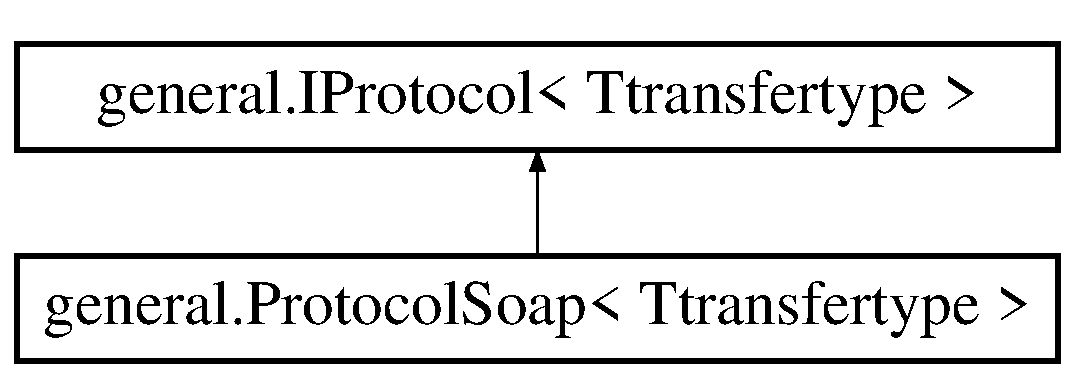
\includegraphics[height=2.000000cm]{classgeneral_1_1_protocol_soap_3_01_ttransfertype_01_4}
\end{center}
\end{figure}
\subsection*{Public Member Functions}
\begin{DoxyCompactItemize}
\item 
{\bf Protocol\-Soap} (int port)
\item 
bool {\bf connect} (Ttransfertype objtype, string url)
\item 
void {\bf disconnect} ()
\item 
bool {\bf send} (Ttransfertype obj)
\end{DoxyCompactItemize}


\subsection{Constructor \& Destructor Documentation}
\index{general\-::\-Protocol\-Soap$<$ Ttransfertype $>$@{general\-::\-Protocol\-Soap$<$ Ttransfertype $>$}!Protocol\-Soap@{Protocol\-Soap}}
\index{Protocol\-Soap@{Protocol\-Soap}!general::ProtocolSoap< Ttransfertype >@{general\-::\-Protocol\-Soap$<$ Ttransfertype $>$}}
\subsubsection[{Protocol\-Soap}]{\setlength{\rightskip}{0pt plus 5cm}general.\-Protocol\-Soap$<$ Ttransfertype $>$.Protocol\-Soap (
\begin{DoxyParamCaption}
\item[{int}]{port}
\end{DoxyParamCaption}
)}\label{classgeneral_1_1_protocol_soap_3_01_ttransfertype_01_4_aa7f80e91f22992527bf0de2f55164bf1}


\subsection{Member Function Documentation}
\index{general\-::\-Protocol\-Soap$<$ Ttransfertype $>$@{general\-::\-Protocol\-Soap$<$ Ttransfertype $>$}!connect@{connect}}
\index{connect@{connect}!general::ProtocolSoap< Ttransfertype >@{general\-::\-Protocol\-Soap$<$ Ttransfertype $>$}}
\subsubsection[{connect}]{\setlength{\rightskip}{0pt plus 5cm}bool general.\-Protocol\-Soap$<$ Ttransfertype $>$.connect (
\begin{DoxyParamCaption}
\item[{Ttransfertype}]{objtype, }
\item[{string}]{url}
\end{DoxyParamCaption}
)}\label{classgeneral_1_1_protocol_soap_3_01_ttransfertype_01_4_a14618cf7ac8a000cca11a1b4ba6771b2}


Implements {\bf general.\-I\-Protocol$<$ Ttransfertype $>$} \doxyref{}{p.}{interfacegeneral_1_1_i_protocol_3_01_ttransfertype_01_4_add439e3269ed0417c7d31f543293cf6d}.

\index{general\-::\-Protocol\-Soap$<$ Ttransfertype $>$@{general\-::\-Protocol\-Soap$<$ Ttransfertype $>$}!disconnect@{disconnect}}
\index{disconnect@{disconnect}!general::ProtocolSoap< Ttransfertype >@{general\-::\-Protocol\-Soap$<$ Ttransfertype $>$}}
\subsubsection[{disconnect}]{\setlength{\rightskip}{0pt plus 5cm}void general.\-Protocol\-Soap$<$ Ttransfertype $>$.disconnect (
\begin{DoxyParamCaption}
{}
\end{DoxyParamCaption}
)}\label{classgeneral_1_1_protocol_soap_3_01_ttransfertype_01_4_a08c49370d9f9c01ddee71446fe2ac072}


Implements {\bf general.\-I\-Protocol$<$ Ttransfertype $>$} \doxyref{}{p.}{interfacegeneral_1_1_i_protocol_3_01_ttransfertype_01_4_a21e9034c26aa630c374af028eb0e1c19}.

\index{general\-::\-Protocol\-Soap$<$ Ttransfertype $>$@{general\-::\-Protocol\-Soap$<$ Ttransfertype $>$}!send@{send}}
\index{send@{send}!general::ProtocolSoap< Ttransfertype >@{general\-::\-Protocol\-Soap$<$ Ttransfertype $>$}}
\subsubsection[{send}]{\setlength{\rightskip}{0pt plus 5cm}bool general.\-Protocol\-Soap$<$ Ttransfertype $>$.send (
\begin{DoxyParamCaption}
\item[{Ttransfertype}]{obj}
\end{DoxyParamCaption}
)}\label{classgeneral_1_1_protocol_soap_3_01_ttransfertype_01_4_aff8117875ae68eb4b55d224e751b8ec1}


Implements {\bf general.\-I\-Protocol$<$ Ttransfertype $>$} \doxyref{}{p.}{interfacegeneral_1_1_i_protocol_3_01_ttransfertype_01_4_afb16cb0284cb948a2af24f2bd5c1b192}.



The documentation for this class was generated from the following file\-:\begin{DoxyCompactItemize}
\item 
general/communication/protocol/{\bf Protocol\-Soap.\-cs}\end{DoxyCompactItemize}

\section{Server.\-Server Class Reference}
\label{class_server_1_1_server}\index{Server.\-Server@{Server.\-Server}}
Inheritance diagram for Server.\-Server\-:\begin{figure}[H]
\begin{center}
\leavevmode
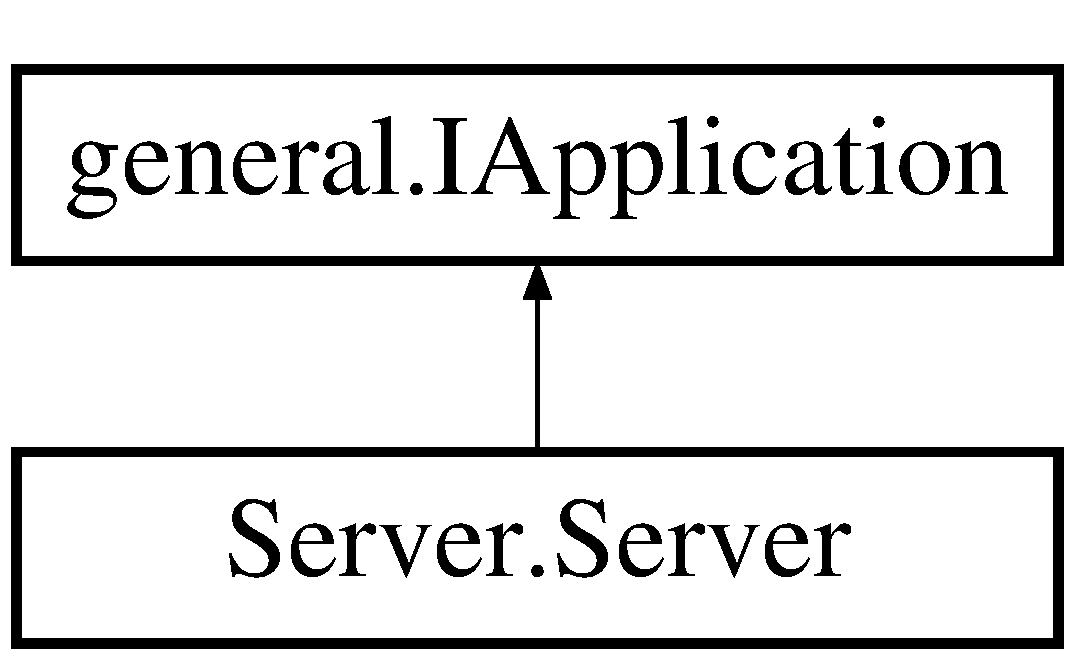
\includegraphics[height=2.000000cm]{class_server_1_1_server}
\end{center}
\end{figure}
\subsection*{Public Member Functions}
\begin{DoxyCompactItemize}
\item 
{\bf Server} ()
\item 
bool {\bf init} ()
\item 
bool {\bf start} ()
\item 
bool {\bf stop} ()
\end{DoxyCompactItemize}


\subsection{Constructor \& Destructor Documentation}
\index{Server\-::\-Server@{Server\-::\-Server}!Server@{Server}}
\index{Server@{Server}!Server::Server@{Server\-::\-Server}}
\subsubsection[{Server}]{\setlength{\rightskip}{0pt plus 5cm}Server.\-Server.\-Server (
\begin{DoxyParamCaption}
{}
\end{DoxyParamCaption}
)}\label{class_server_1_1_server_a77c4d462bec0f11da1fff5166c54b521}


\subsection{Member Function Documentation}
\index{Server\-::\-Server@{Server\-::\-Server}!init@{init}}
\index{init@{init}!Server::Server@{Server\-::\-Server}}
\subsubsection[{init}]{\setlength{\rightskip}{0pt plus 5cm}bool Server.\-Server.\-init (
\begin{DoxyParamCaption}
{}
\end{DoxyParamCaption}
)}\label{class_server_1_1_server_afb8a142170af0d8758ca23875bc93d69}
Initialize Application object +\-Do any pre setting up before application starts +\-Should include things not critical to the creation of the object. 

Implements {\bf general.\-I\-Application} \doxyref{}{p.}{interfacegeneral_1_1_i_application_a0b53a00ac509c31efcc46fe5d20c156f}.

\index{Server\-::\-Server@{Server\-::\-Server}!start@{start}}
\index{start@{start}!Server::Server@{Server\-::\-Server}}
\subsubsection[{start}]{\setlength{\rightskip}{0pt plus 5cm}bool Server.\-Server.\-start (
\begin{DoxyParamCaption}
{}
\end{DoxyParamCaption}
)}\label{class_server_1_1_server_a161ab2103af04dcdd6d00645a3072d30}
Start application 

Implements {\bf general.\-I\-Application} \doxyref{}{p.}{interfacegeneral_1_1_i_application_a44ef333a6aefd814ef4db3f04a45b5e1}.

\index{Server\-::\-Server@{Server\-::\-Server}!stop@{stop}}
\index{stop@{stop}!Server::Server@{Server\-::\-Server}}
\subsubsection[{stop}]{\setlength{\rightskip}{0pt plus 5cm}bool Server.\-Server.\-stop (
\begin{DoxyParamCaption}
{}
\end{DoxyParamCaption}
)}\label{class_server_1_1_server_a84955f96214411a79da90cd2acfd7e2d}
Stop application +\-Should return true on successful stop. +\-Should only stop if application is not busy, in this case return false. 

Implements {\bf general.\-I\-Application} \doxyref{}{p.}{interfacegeneral_1_1_i_application_a497ef4a13f7f98a1a7656c529933fa53}.



The documentation for this class was generated from the following file\-:\begin{DoxyCompactItemize}
\item 
server/{\bf server.\-cs}\end{DoxyCompactItemize}

\section{general.\-Server\-Client$<$ Ttransfertype $>$ Class Template Reference}
\label{classgeneral_1_1_server_client_3_01_ttransfertype_01_4}\index{general.\-Server\-Client$<$ Ttransfertype $>$@{general.\-Server\-Client$<$ Ttransfertype $>$}}
Inheritance diagram for general.\-Server\-Client$<$ Ttransfertype $>$\-:\begin{figure}[H]
\begin{center}
\leavevmode
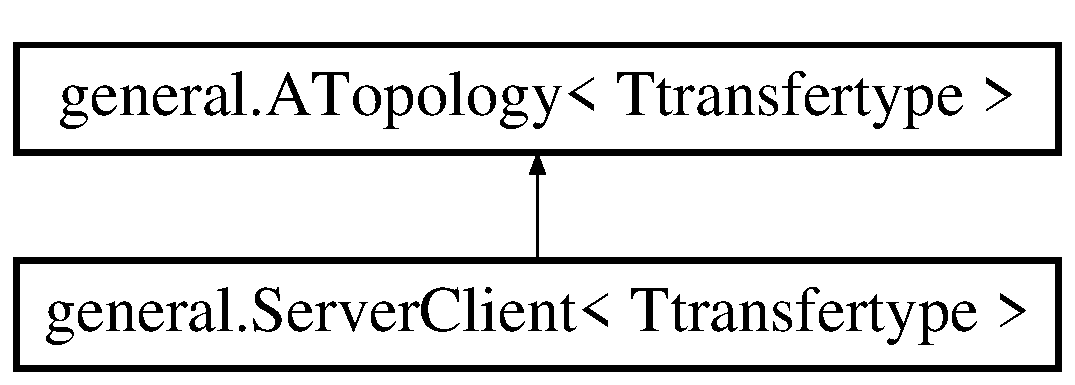
\includegraphics[height=2.000000cm]{classgeneral_1_1_server_client_3_01_ttransfertype_01_4}
\end{center}
\end{figure}
\subsection*{Public Member Functions}
\begin{DoxyCompactItemize}
\item 
{\bf Server\-Client} (I\-Protocol$<$ Ttransfertype $>$ {\bf protocol})
\item 
override bool {\bf connect} (Ttransfertype obj)
\item 
override void {\bf disconnect} ()
\end{DoxyCompactItemize}
\subsection*{Additional Inherited Members}


\subsection{Constructor \& Destructor Documentation}
\index{general\-::\-Server\-Client$<$ Ttransfertype $>$@{general\-::\-Server\-Client$<$ Ttransfertype $>$}!Server\-Client@{Server\-Client}}
\index{Server\-Client@{Server\-Client}!general::ServerClient< Ttransfertype >@{general\-::\-Server\-Client$<$ Ttransfertype $>$}}
\subsubsection[{Server\-Client}]{\setlength{\rightskip}{0pt plus 5cm}general.\-Server\-Client$<$ Ttransfertype $>$.Server\-Client (
\begin{DoxyParamCaption}
\item[{I\-Protocol$<$ Ttransfertype $>$}]{protocol}
\end{DoxyParamCaption}
)}\label{classgeneral_1_1_server_client_3_01_ttransfertype_01_4_a9a3c49921544145f2c2f3c6576e455d3}


\subsection{Member Function Documentation}
\index{general\-::\-Server\-Client$<$ Ttransfertype $>$@{general\-::\-Server\-Client$<$ Ttransfertype $>$}!connect@{connect}}
\index{connect@{connect}!general::ServerClient< Ttransfertype >@{general\-::\-Server\-Client$<$ Ttransfertype $>$}}
\subsubsection[{connect}]{\setlength{\rightskip}{0pt plus 5cm}override bool general.\-Server\-Client$<$ Ttransfertype $>$.connect (
\begin{DoxyParamCaption}
\item[{Ttransfertype}]{obj}
\end{DoxyParamCaption}
)\hspace{0.3cm}{\ttfamily [virtual]}}\label{classgeneral_1_1_server_client_3_01_ttransfertype_01_4_ac79cb3704b830ad1436bb18b48ed5755}


Implements {\bf general.\-A\-Topology$<$ Ttransfertype $>$} \doxyref{}{p.}{classgeneral_1_1_a_topology_3_01_ttransfertype_01_4_ad98d6292318094e2f8e6008324adb6b6}.

\index{general\-::\-Server\-Client$<$ Ttransfertype $>$@{general\-::\-Server\-Client$<$ Ttransfertype $>$}!disconnect@{disconnect}}
\index{disconnect@{disconnect}!general::ServerClient< Ttransfertype >@{general\-::\-Server\-Client$<$ Ttransfertype $>$}}
\subsubsection[{disconnect}]{\setlength{\rightskip}{0pt plus 5cm}override void general.\-Server\-Client$<$ Ttransfertype $>$.disconnect (
\begin{DoxyParamCaption}
{}
\end{DoxyParamCaption}
)\hspace{0.3cm}{\ttfamily [virtual]}}\label{classgeneral_1_1_server_client_3_01_ttransfertype_01_4_a39edc8a7d4acc3c36baee5b90be87423}


Implements {\bf general.\-A\-Topology$<$ Ttransfertype $>$} \doxyref{}{p.}{classgeneral_1_1_a_topology_3_01_ttransfertype_01_4_ad51a3927e211946711c52f368ce21301}.



The documentation for this class was generated from the following file\-:\begin{DoxyCompactItemize}
\item 
general/communication/topology/{\bf Server\-Client.\-cs}\end{DoxyCompactItemize}

\chapter{File Documentation}
\section{client/client.cs File Reference}
\label{client_8cs}\index{client/client.\-cs@{client/client.\-cs}}
\subsection*{Classes}
\begin{DoxyCompactItemize}
\item 
class {\bf client.\-client}
\end{DoxyCompactItemize}
\subsection*{Namespaces}
\begin{DoxyCompactItemize}
\item 
package {\bf client}
\end{DoxyCompactItemize}
\subsection*{Constant Groups}
\begin{DoxyCompactItemize}
\item 
package {\bf client}
\end{DoxyCompactItemize}

\section{client/client\-G\-U\-I.cs File Reference}
\label{client_g_u_i_8cs}\index{client/client\-G\-U\-I.\-cs@{client/client\-G\-U\-I.\-cs}}
\subsection*{Classes}
\begin{DoxyCompactItemize}
\item 
interface {\bf client.\-client\-G\-U\-I}
\end{DoxyCompactItemize}
\subsection*{Namespaces}
\begin{DoxyCompactItemize}
\item 
package {\bf client}
\end{DoxyCompactItemize}
\subsection*{Constant Groups}
\begin{DoxyCompactItemize}
\item 
package {\bf client}
\end{DoxyCompactItemize}

\section{general/\-A\-Computer.cs File Reference}
\label{_a_computer_8cs}\index{general/\-A\-Computer.\-cs@{general/\-A\-Computer.\-cs}}
\subsection*{Classes}
\begin{DoxyCompactItemize}
\item 
class {\bf general.\-A\-Computer$<$ Tprinter, Tuser $>$}
\end{DoxyCompactItemize}
\subsection*{Namespaces}
\begin{DoxyCompactItemize}
\item 
package {\bf general}
\end{DoxyCompactItemize}
\subsection*{Constant Groups}
\begin{DoxyCompactItemize}
\item 
package {\bf general}
\end{DoxyCompactItemize}

\section{general/communication/protocol/\-I\-Protocol.cs File Reference}
\label{_i_protocol_8cs}\index{general/communication/protocol/\-I\-Protocol.\-cs@{general/communication/protocol/\-I\-Protocol.\-cs}}
\subsection*{Classes}
\begin{DoxyCompactItemize}
\item 
interface {\bf general.\-I\-Protocol$<$ Ttransfertype $>$}
\end{DoxyCompactItemize}
\subsection*{Namespaces}
\begin{DoxyCompactItemize}
\item 
package {\bf general}
\end{DoxyCompactItemize}
\subsection*{Constant Groups}
\begin{DoxyCompactItemize}
\item 
package {\bf general}
\end{DoxyCompactItemize}

\section{general/communication/protocol/\-Protocol\-Soap.cs File Reference}
\label{_protocol_soap_8cs}\index{general/communication/protocol/\-Protocol\-Soap.\-cs@{general/communication/protocol/\-Protocol\-Soap.\-cs}}
\subsection*{Classes}
\begin{DoxyCompactItemize}
\item 
class {\bf general.\-Protocol\-Soap$<$ Ttransfertype $>$}
\end{DoxyCompactItemize}
\subsection*{Namespaces}
\begin{DoxyCompactItemize}
\item 
package {\bf general}
\end{DoxyCompactItemize}
\subsection*{Constant Groups}
\begin{DoxyCompactItemize}
\item 
package {\bf general}
\end{DoxyCompactItemize}

\section{general/communication/topology/\-Atopology.cs File Reference}
\label{_atopology_8cs}\index{general/communication/topology/\-Atopology.\-cs@{general/communication/topology/\-Atopology.\-cs}}
\subsection*{Classes}
\begin{DoxyCompactItemize}
\item 
class {\bf general.\-A\-Topology$<$ Ttransfertype $>$}
\end{DoxyCompactItemize}
\subsection*{Namespaces}
\begin{DoxyCompactItemize}
\item 
package {\bf general}
\end{DoxyCompactItemize}
\subsection*{Constant Groups}
\begin{DoxyCompactItemize}
\item 
package {\bf general}
\end{DoxyCompactItemize}

\section{general/communication/topology/\-Server\-Client.cs File Reference}
\label{_server_client_8cs}\index{general/communication/topology/\-Server\-Client.\-cs@{general/communication/topology/\-Server\-Client.\-cs}}
\subsection*{Classes}
\begin{DoxyCompactItemize}
\item 
class {\bf general.\-Server\-Client$<$ Ttransfertype $>$}
\end{DoxyCompactItemize}
\subsection*{Namespaces}
\begin{DoxyCompactItemize}
\item 
package {\bf general}
\end{DoxyCompactItemize}
\subsection*{Constant Groups}
\begin{DoxyCompactItemize}
\item 
package {\bf general}
\end{DoxyCompactItemize}

\section{general/\-Computer.cs File Reference}
\label{_computer_8cs}\index{general/\-Computer.\-cs@{general/\-Computer.\-cs}}
\subsection*{Classes}
\begin{DoxyCompactItemize}
\item 
class {\bf general.\-Computer}
\end{DoxyCompactItemize}
\subsection*{Namespaces}
\begin{DoxyCompactItemize}
\item 
package {\bf general}
\end{DoxyCompactItemize}
\subsection*{Constant Groups}
\begin{DoxyCompactItemize}
\item 
package {\bf general}
\end{DoxyCompactItemize}

\section{general/\-I\-Application.cs File Reference}
\label{_i_application_8cs}\index{general/\-I\-Application.\-cs@{general/\-I\-Application.\-cs}}
\subsection*{Classes}
\begin{DoxyCompactItemize}
\item 
interface {\bf general.\-I\-Application}
\end{DoxyCompactItemize}
\subsection*{Namespaces}
\begin{DoxyCompactItemize}
\item 
package {\bf general}
\end{DoxyCompactItemize}
\subsection*{Constant Groups}
\begin{DoxyCompactItemize}
\item 
package {\bf general}
\end{DoxyCompactItemize}

\section{general/\-I\-Printer.cs File Reference}
\label{_i_printer_8cs}\index{general/\-I\-Printer.\-cs@{general/\-I\-Printer.\-cs}}
\subsection*{Classes}
\begin{DoxyCompactItemize}
\item 
interface {\bf I\-Printer$<$ Ttasktype, Tstate $>$}
\end{DoxyCompactItemize}

\section{general/\-I\-Print\-Task.cs File Reference}
\label{_i_print_task_8cs}\index{general/\-I\-Print\-Task.\-cs@{general/\-I\-Print\-Task.\-cs}}
\subsection*{Classes}
\begin{DoxyCompactItemize}
\item 
interface {\bf general.\-I\-Print\-Task}
\end{DoxyCompactItemize}
\subsection*{Namespaces}
\begin{DoxyCompactItemize}
\item 
package {\bf general}
\end{DoxyCompactItemize}
\subsection*{Constant Groups}
\begin{DoxyCompactItemize}
\item 
package {\bf general}
\end{DoxyCompactItemize}

\section{general/\-Printer.cs File Reference}
\label{_printer_8cs}\index{general/\-Printer.\-cs@{general/\-Printer.\-cs}}
\subsection*{Classes}
\begin{DoxyCompactItemize}
\item 
class {\bf general.\-Printer}
\end{DoxyCompactItemize}
\subsection*{Namespaces}
\begin{DoxyCompactItemize}
\item 
package {\bf general}
\end{DoxyCompactItemize}
\subsection*{Constant Groups}
\begin{DoxyCompactItemize}
\item 
package {\bf general}
\end{DoxyCompactItemize}

\section{general/\-Print\-Task.cs File Reference}
\label{_print_task_8cs}\index{general/\-Print\-Task.\-cs@{general/\-Print\-Task.\-cs}}
\subsection*{Classes}
\begin{DoxyCompactItemize}
\item 
class {\bf general.\-Print\-Task}
\end{DoxyCompactItemize}
\subsection*{Namespaces}
\begin{DoxyCompactItemize}
\item 
package {\bf general}
\end{DoxyCompactItemize}
\subsection*{Constant Groups}
\begin{DoxyCompactItemize}
\item 
package {\bf general}
\end{DoxyCompactItemize}

\section{general/\-Properties/\-Assembly\-Info.cs File Reference}
\label{_assembly_info_8cs}\index{general/\-Properties/\-Assembly\-Info.\-cs@{general/\-Properties/\-Assembly\-Info.\-cs}}

\section{main.\-cs File Reference}
\label{main_8cs}\index{main.\-cs@{main.\-cs}}
\subsection*{Classes}
\begin{DoxyCompactItemize}
\item 
class {\bf Printing.\-Printing}
\end{DoxyCompactItemize}
\subsection*{Namespaces}
\begin{DoxyCompactItemize}
\item 
package {\bf Printing}
\end{DoxyCompactItemize}
\subsection*{Constant Groups}
\begin{DoxyCompactItemize}
\item 
package {\bf Printing}
\end{DoxyCompactItemize}

\section{server/server.cs File Reference}
\label{server_8cs}\index{server/server.\-cs@{server/server.\-cs}}
\subsection*{Classes}
\begin{DoxyCompactItemize}
\item 
class {\bf Server.\-Server}
\end{DoxyCompactItemize}
\subsection*{Namespaces}
\begin{DoxyCompactItemize}
\item 
package {\bf Server}
\end{DoxyCompactItemize}
\subsection*{Constant Groups}
\begin{DoxyCompactItemize}
\item 
package {\bf Server}
\end{DoxyCompactItemize}

%--- End generated contents ---

% Index
\newpage
\phantomsection
\addcontentsline{toc}{part}{Index}
\printindex

\end{document}
